\section{NAO - The Humanoid Robot} NAO is an autonomous programmable humanoid robot invented by Aldebaran Robotics. NAO Academics Edition was developed for universities and laboratories for research and educational purposes. Follow subsections discuss briefly about the specifications of NAO as described by Aldebaran Robotics.

\begin{table}
	[h] \centering \caption{NAO V5 specification } \label{tb:nao:spec} 
	\begin{tabular}
		{|l|l|} \hline Height & 58 centimetres (23 in) \\
		\hline Weight & 4.3 kilograms (9.5 lb) \\
		\hline Battery autonomy & 60 minutes (active use), 90 minutes (normal use) \\
		\hline Degrees of freedom & 21 to 25 \\
		\hline CPU & Intel Atom @ 1.6 GHz \\
		\hline Built-in OS & Linux \\
		\hline SDK compatibility & Windows, Mac OS, Linux \\
		\hline Programming languages & C++, Python, Java, MATLAB, Urbi, C, .Net \\
		\hline Vision & 2 x HD 1280x960 cameras \\
		\hline Connectivity & Ethernet, Wi-Fi \\
		\hline \multirow{6}{*}{Sensors} & 4 x directional microphones \\
		& 1 x sonar rangefinder \\
		& 2 x IR emitters and receivers \\
		& 1 x inertial board \\
		& 9 x tactile sensors \\
		& 8 x pressure sensors \\
		\hline 
	\end{tabular}
\end{table}


\subsection{Construction} NAO has a body with 25 degrees of freedom (DOF) whose key elements are electric motors and actuators as show in the figure \ref{fg:nao:construction}. It has 48.6-watt-hour battery that provides NAO with 1.5 or more hours of autonomy, depending on usage. Additional specifications of NAO are shown in the table \ref{tb:nao:spec}. ---- Add more info ----

\begin{figure}
	[h] \centering 
	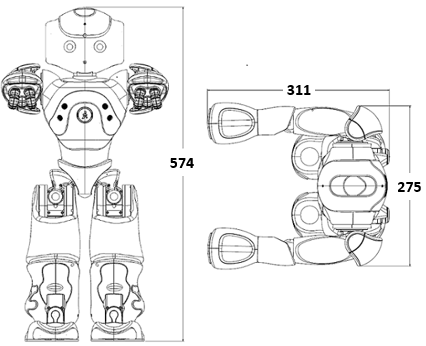
\includegraphics[height=7cm]{figures/content/nao-construction.png} \caption{Construction of NAO} \label{fg:nao:construction} 
\end{figure}


\subsection{Motion} NAOs walking algorithm uses a simple dynamic model (linear inverse pendulum) and quadratic programming. It is stabilized using feedback from joint sensors. This makes the walking robust and resistant to small disturbances, and torso oscillations in the frontal and lateral planes are absorbed. It can walk on a variety of floor surfaces, such as carpeted, tiled, and wooden floors. 

NAOs motion module is based on generalized inverse kinematics, which handles Cartesian coordinates, joint control, balance, redundancy, and task priority. This means that when asking it to extend its arm, it bends over because its arms and leg joints are taken into account.

\begin{figure}
	\centering 
	\begin{minipage}
		{.3 
		\textwidth} \centering 
		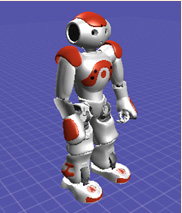
\includegraphics[height=5cm]{/content/nao-stand.jpg} 
	\end{minipage}
	\begin{minipage}
		{.3 
		\textwidth} \centering 
		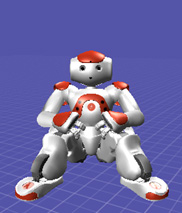
\includegraphics[height=5cm]{/content/nao-sit.jpg} 
	\end{minipage}
	\begin{minipage}
		{.3 
		\textwidth} \centering 
		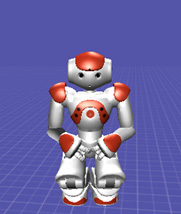
\includegraphics[height=5cm]{/content/nao-crouch.jpg} 
	\end{minipage}
	\caption{Standing, Sitting and Crouching postures of virtual NAO using ALRobotPosture module. \cite{8}} \label{fg:nao:motion} 
\end{figure}


In this thesis, we used locomotion and stiffness control of Motion API to move NAO to a position in the two dimensional space. Robot Posture API was also used to make the robot go to the predefined posture such as Stand, Sit and Crouch as shown in the figure \ref{fg:nao:motion}. Python code \ref{code:nao:motion} shows how the robot can be moved to another position at the given normalized velocity using Motion API. 

\lstinputlisting[language=python]{code/nao-motion.py} \label{code:nao:motion}

\subsection{Audio} NAO uses four directional microphones to detect sounds and equipped with a stereo broadcast system made up of 2 loudspeakers in its ears as shown in the figure \ref{fg:nao:audio}. NAOs voice recognition and text-to-speech capabilities allow it to communicate in 19 languages. 

\begin{figure}
	[h] \centering 
	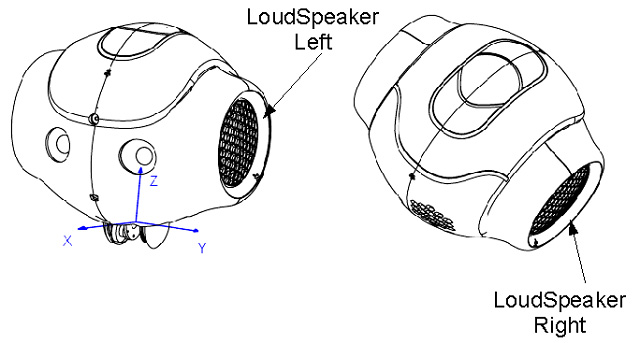
\includegraphics[height=7cm]{figures/content/nao-audio.jpg} \caption{NAO Audio} \label{fg:nao:audio} 
\end{figure}
 

In this thesis, we used Text-To-Speech API of NAO to say some words loud to communicate with the user.Python code \ref{code:nao:audio} shows how NAO can say words given as strings.

\lstinputlisting[language=python]{code/nao-audio.py} \label{code:nao:audio}

\subsection{Vision}
Proper vision is the utmost importance for the function of any vision based autonomous robot. Areas of artificial intelligence deal with autonomous planning or deliberation for robotic systems to navigate through an environment. A detailed understanding of these environments is required to navigate through them. High-level information about the environment could be provided by a computer vision system that is acting as a vision sensor.

 Two identical video RGB cameras are located in the forehead of NAO as shown in the figure \ref{fg:nao:vision}. They provide up to 1280x960 resolution at 30 frames per second. NAO contains a set of algorithms for detecting and recognizing faces and shapes.

\begin{figure}
	[h] \centering 
	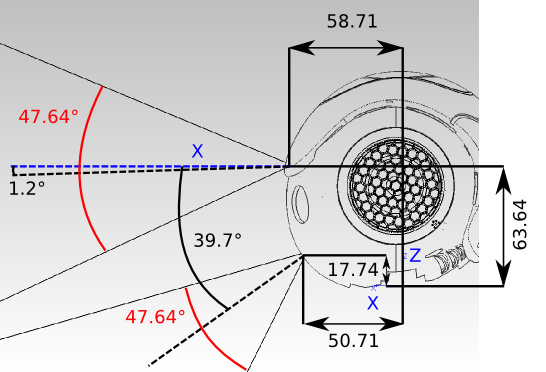
\includegraphics[height=7cm]{figures/content/nao-vision.jpg} \caption{The field of view of two identical RGB video cameras which are located in the forehead of NAO. \cite{8} } \label{fg:nao:vision} 
\end{figure}


Skeletal points based gesture recognition needs three dimensional data of the human bone joints. However, sensors integrated with NAO could not provide precise three dimensional data for processing heavy algorithms to track human skeletal joints. 3D cameras such as Microsoft Kinect and Asus Xtion are used not only for gaming but also for analyzing 3D data, including algorithms for feature selection, scene analysis, motion tracking, skeletal tracking and gesture recognition \cite{12}. 

Asus Xtion PRO LIVE uses infrared sensors, adaptive depth detection technology, color image sensing and audio stream to capture a user's real-time image, movement, and voice, making user tracking more precise. 

\begin{figure}
	[h] \centering 
	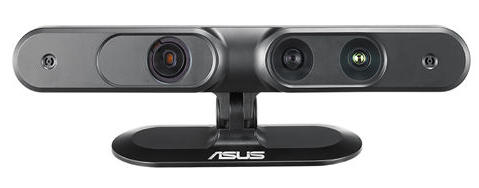
\includegraphics[height=4cm]{figures/content/xtion.png} 
	\caption{Asus Xtion Pro Live}
	\label{fg:xtion} 
\end{figure}

Therefore in this thesis, we attempted to use Asus Xtion PRO LIVE as an external camera that was mounted on the head of NAO as shown in the figure \ref{fg:xtion}. 

\begin{figure}
	[h] \centering 
	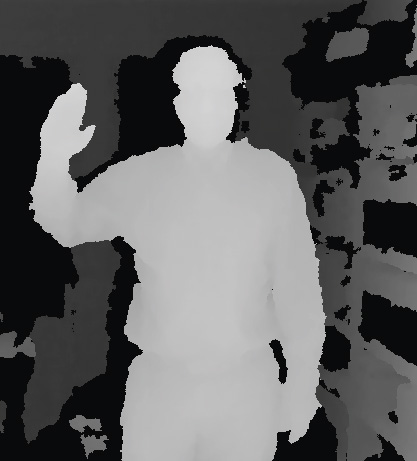
\includegraphics[height=8cm]{figures/content/xtion-depth.jpg} 	
	\caption{Depth Image recorded by depth camera Asus Xtion Pro Live} \label{fg:xtion:depth} 
\end{figure}


--- this section needs revision ---

\subsection{Computing} NAO is equipped with Intel ATOM 1.6 GHz CPU in the head that runs a 32 bit Gentoo Linux to support Aldebarans proprietary middleware (NAOqi). NAOqi Framework is the programming framework used to program Aldebaran robots. This framework allows homogeneous communication between different modules such as motion, audio, video. NAOqi executable which runs on the robot is a broker. The broker provides lookup services so that any module in the tree or across the network can find any method that has been advertised.

\begin{figure}
	[h] \centering 
	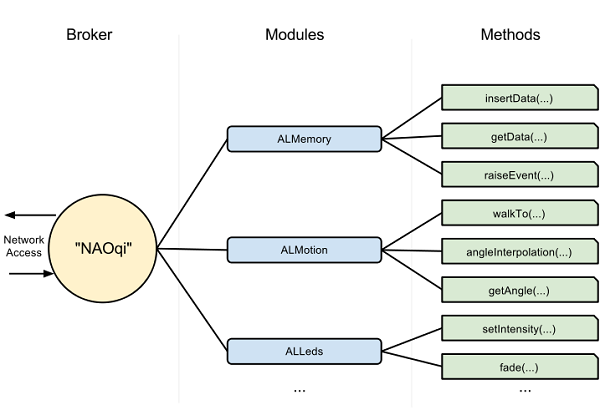
\includegraphics[height=7cm]{figures/content/nao-proxy.png} 
	\caption{NAOqi Proxy}
	\label{fg:nao:proxy} 
\end{figure}

Computational limitations of NAOs CPU hinders us to build a real time gesture recognition based on human skeletal joints. Therefore, we used an off-board computer to execute the gesture recognition program and communicated with NAO via NAOqi proxies. 
